\begin{figure}
\begin{center}
    %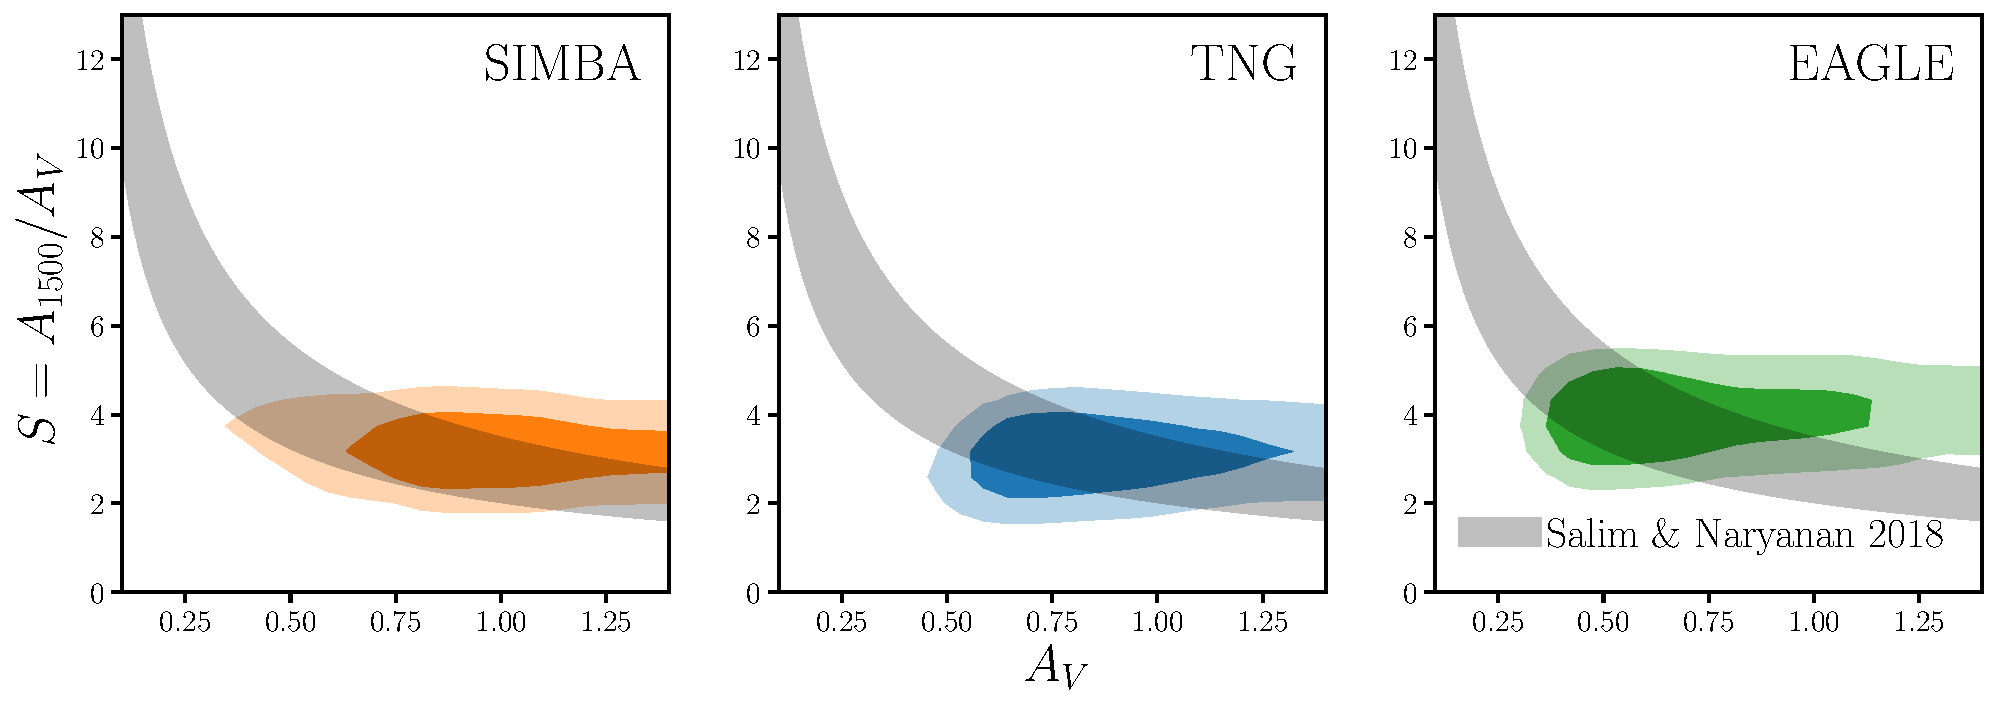
\includegraphics[width=0.9\textwidth]{figs/abc_slope_AV_starforming.pdf}
    \caption{\label{fig:slope}
    The attenuation-slope relation of star-forming galaxies ($\ssfr >
    10^{-11}yr^{-1}$), using the attenuation curves predicted by our  
    \eda~prescription for the median posterior parameter values of SIMBA
    (left), TNG (center) and EAGLE (right). 
    For comparison, we include the observed attenuation-slope relation
    from GSWLC2~\citep{salim2020}. 
    We use $A_V$ and $S = A(1500\AA)/A_V$ as measurements of attenuation and
    slope, respectively. 
    \chedit{
        \emph{The \eda~does not predict $A_V < 0.3$ because star-forming galaxies in
        the simulations are too lumnious and require significant attenuation to
        reproduce observations.}
        Beyond $A_V > 0.3$, however, there is good agreement between the
        attenuation-slope relation predicted by the \eda~and observations. 
    }
    }
\end{center}
\end{figure}

\subsection{Comparison to Dust Observations} \label{sec:reproduce}
With our \eda~prescription, we are able to accurately reproduce the
observed optical and UV color-magnitude relations with our simulations. 
In addition to  reproducing observations, since the \eda~assigns dust
attenuation curves to each simulated galaxy, we can compare the
\eda~attenuation curves to dust attenuation measured from
observations. 
We begin with the well-established attenuation-slope relation: star-forming
galaxies with higher dust attenuation have shallower attenuation curves. 
This relation is a consequence of dust scattering dominating absorption at
low attenuation while dust absorption dominates at high
attenuation~\citep{gordon1994, witt2000, draine2003, chevallard2013}. 
In Figure~\ref{fig:slope}, we present the attenuation-slope relation of
star-forming galaxies with $\ssfr > 10^{-11}yr^{-1}$ based on the
dust attenuation curves predicted by the \eda~for the median posteriors of
SIMBA (left), TNG (center) and EAGLE (right).
For comparison, we include the observed attenuation-slope relations of
GSWLC2 galaxies~\citep[grey shaded;][]{salim2020}.
For attenuation we use $A_V$ and for slope we use the UV-optical slope, $S
= A(1500\AA)/A_V$, commonly found in the literature. 
The contours mark the 68 and 95 percentiles. 
Most noticably, we find that the \eda~does not predict $A_V < 0.3$. 
\chedit{
    This is not due to the selection function imposed by our forward model. 
    The attenuation-slope relation of star-forming galaxies in GSWLC2 does not
    change significantly if we impose similar selection cuts as our
    observational sample.
    Instead, the lack of star-forming galaxies with $A_V < 0.3$ is a
    consequence of SIMBA, TNG, and EAGLE predicting star-forming galaxies that
    are more luminous than observations.  
}
All of the simulations have star-forming galaxies with intrinsic $M_r <
-21$ and $\gr < 0.5$ (Figure~\ref{fig:obs}). 
This is further corroborated by the $\sfr-M*$ relations in
Figure~\ref{fig:smf_msfr}, where the simulations all have star-forming
galaxies with $M_* > 10^{11}M_\odot$, not found in SDSS. 
To reproduce the SDSS optical color-magnitude relation these galaxies would
need to be significantly reddened and attenuated. 
Hence, any dust prescription for the simulations would require high 
$A_V$ for star-forming galaxies.
Nevertheless, for $A_V > 0.3$, we find good agreement between the 
attenuation-slope relation predicted by the \eda~and observations. 
\chedit{
    We also note that $A_V$ values can vary {\em significantly} between
    different measurements --- even for the same galaxy. 
    SDSS star-forming galaxies, for instance, have significantly higher 
    $A_V > 0.3$ according to the \cite{brinchmann2004} measurements
    (Appendix~\ref{sec:slab}).
}

%We note that the difference in the $A_V$ ranges is due to the $M_r$
%completeness limit imposed by our forward model (Section~\ref{sec:fm}).
%The GSWLC2 sample in \cite{salim2020} extends down to $M_* \sim
%10^{8.5}M_\odot$; however, the TNG and EAGLE samples do not extend below
%$M_* \sim10^{10}M_\odot$.
%\emph{The \eda~predicts attenuation-slope relations for TNG and EAGLE that
%are in excellent agreement with observations.} 

\begin{figure}
\begin{center}
    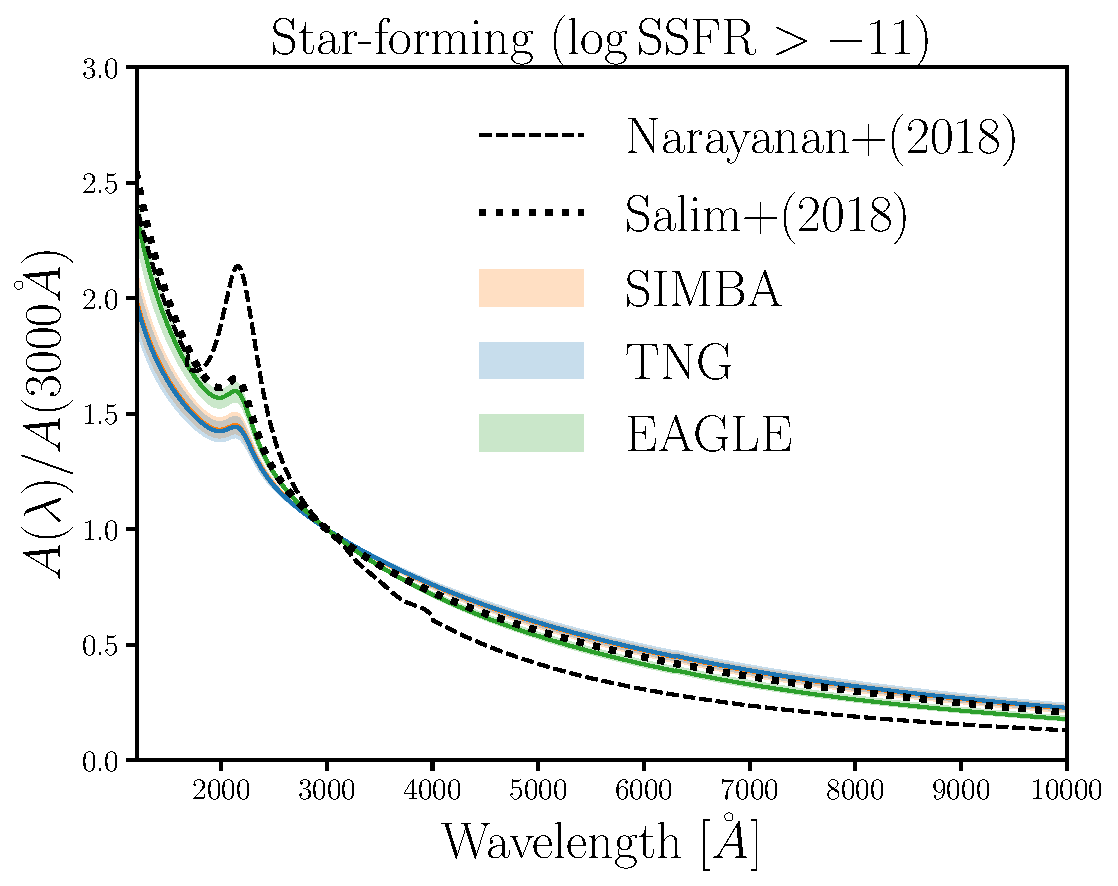
\includegraphics[width=0.5\textwidth]{figs/abc_sf_attenuation.pdf}
    \caption{\label{fig:sfatten}
    The normalized attenuation curves of star-forming galaxies predicted by
    the \eda~for median posterior parameter values of SIMBA (orange), TNG
    (blue), and EAGLE (green).  
    Galaxies with $\log \ssfr > -11~yr^{-1}$ are classified as star-forming. 
    The attenuation curves are normalized at $3000\AA$ and we mark the
    68 percentile of the attenuation curves with the shaded region.
    For comparison, we include $A(\lambda)/A(3000\AA)$ measurements from
    the~\cite{narayanan2018} radiative transfer simulation (dashed) and
    \cite{salim2018} observations (dotted).
    %The \cite{calzetti2000} and \cite{battisti2017} attenuation curves are shallower than the \eda~attenuation curves; however, they probe lower $M_*$ galaxies than our forward modeled TNG and EAGLE samples.  For attenuation curve from \cite{salim2018}, which probe a similar $M_*$ range, we find goood agreement. 
    {\em The \eda~predict attenuation curves of star-forming galaxies that
    are in good agreement with the attenuation curves measured from
    the simulation and observations in the literature.}
    %We also find good agreement with median attenuation curve of star-forming galaxies in the radiative transfer simulations of \cite{narayanan2018}.
    }
\end{center}
\end{figure}

In addition to the attenuation-slope relation, we can also directly compare
the attenuation curves predicted by the \eda~to measurements from
observations for star-forming galaxies. 
In Figure~\ref{fig:sfatten}, we present the normalized attenuation curves
of star-forming galaxies predicted by the \eda~for the median posterior
parameter values of SIMBA(orange), TNG (blue), and EAGLE (green).
We again define galaxies with $\ssfr > 10^{-11}{yr}^{-1}$ as star-forming.
The attenuation curves are normalized at $3000\AA$ and we present the
variation in the attenuation curves in the shaded region, 68 percentile. 
For comparison, we include $A(\lambda)/A(3000\AA)$ from the
\cite{narayanan2018} radiative transfer simulation (dashed) and 
observations~\citep[][dotted]{salim2018}. 
The attenuation curve from \cite{salim2018} corresponds to star-forming
galaxies with $M_* > 10^{10.5}M_\odot$, a similar $M_*$ range as our
forward modeled samples. 
Since we do not vary the UV bump in our \eda~prescription, we ignore any
discrepancies in the amplitudes of the bump. 
\emph{Overall, we find good agreement between the \eda~attenuation curves for
star-forming galaxies and the attenuation curves from observations and
simulations in the literature.}

%Again, the fact that we reproduce the detailed dust attenuation curves of star-forming galaxies in observations and simulations with the \eda~without fitting for them, highlights the advantages of a forward modeling approach. 

%The \eda~attenuation curves are slightly steeper than the \cite{calzetti2000} and \cite{battisti2017} curves. 
%These attenuation curves, however, are derived from $M_* < 10^{9.9}M_\odot$
%star-forming galaxies, which lie below the $M_*$ limit of our forward
%modeled TNG and EAGLE samples. 
%Meanwhile, the TNG and EAGLE \eda~attenuation curves are in good agreement
%with the \cite{salim2018} attenuation curve for $M_* > 10^{10.5}M_\odot$ star-forming galaxies. 
%They are also consistent with the median curve of \cite{narayanan2018}. 

%The \eda~attenuation curves are noticeably steeper than the \cite{calzetti2000} and \cite{battisti2017} curves.  These attenuation curves, however, are derived from $M_* < 10^{9.9}M_\odot$ star-forming galaxies --- below our $M_*$ range. 
%Since we find $\mdeltam < 0$ for both the TNG and EAGLE posteriors, the \eda~attenuation curves are consistent with \cite{calzetti2000} and \cite{battisti2017}. 


%\chedit{ 
%    The \eda~predicts higher dust attenuation at lower wavelenghts for
%    star-forming galaxies.
%    Without dust attenuation, both TNG and EAGLE predict star-forming galaxies
%    that are bluer in the optical and UV than observations
%    (Figure~\ref{fig:obs}).
%    To reproduce the SDSS, the \eda~significantly reddens star-forming galaxies.
%}
%In Figure~\ref{fig:raw_atten}, we also find that more massive star-forming
%galaxies have higher attenuation. This is because the simulations overpredict 
%luminous blue star-forming galaxies, which must be attenuated to reproduce
%observations. 


%At low attenuation, dust scattering dominates absoprtion so the 
%attenuation curve steepens because red light scatters isotropically while blue light
%scatters forward~\citep{gordon1994, witt2000, draine2003}. %, which causes more optical-to-IR light to escape the galaxy than UV light
%At high attenuation dust absorption is dominant and the attenuation curve is
%shallower~\citep{chevallard2013}. For the $A_V$ range probed by the DEM, the
%$A_V$--slope relation is in good agreement with GSWLC2 galaxies~\citep[black shaded][]{salim2020}.
%They are also consistent with \cite{leja2017}. We also compare our results to
%theoretical predictions from radiative transfer models, \cite{inoue2005}
%(dotted), the radiative transfer models considered in \cite{chevallard2013}
%(dot dashed), and \cite{trayford2020} (light shaded), which all predict shallower 
%attenuation curves than observations. This is also the case for the
%\cite{narayanan2018} attenuation curves (not included). 
%\emph{The attenuation curve slopes from the DEM for are in excellent
%agreement with observations and better reproduces the observed
%attenuation--slope relation than radiative transfer models.}
